\label{Realisierung}
\chapter{Realisierung}


    \section{Telegram Bot Framwork}

        \subsection{Generierung Telegram Bot}

            Als ersten Schritt zur Erschaffung eines Telegram-Bots wird der Bot-Father (selbst ein Telegram-Bot \cite{coreTelegram}) konsultiert.  Er erstellt das Framework, registriert den Bot und gibt ein API-Token zurück, das verwendet werden kann, um sich gegenüber der Telegram-Bot-API als Entwickler zu identifizieren. \cite{telegramAPI}


        \section{Vanilla Bot Implementierung}
            Als Basis (boiler plate) für den Coaching Bot (fortan \glqq Bot\grqq) nutzen wir die breit in der Community abgestütze Implementierung \textbf{Conversation Bot} \cite{conversationBot}. Sie stellt uns die basale Anbindung an die State Machine zur Verfügung und ist einfach genug, um als Einstieg in einen vordefinierten Bot zu fungieren. Im Gegensatz dazu ist der \glqq Nested Converation Bot\grqq  schon zu umfangreich und zu mächtig für unsere Zwecke.

            Die Kommunikationslogik des Bots basiert auf einer State Machine. Die Zustände, in denen der Bot sich befinden kann, sind vordefiniert und immer mit einer Aktion und einer Reaktion verbunden. Aktionen werden meist von Seiten des Benutzers durch eine Eingabe oder einen Befehl ausgelöst. Reaktionen sind in Funktionen vordefiniert. Deren Umfang wird im Folgenden funktional und in \ref{Implementierung} Implementierung technisch beschrieben.

    
    \section{Meta-Funktionen}
        Neben den Hauptfunktionen des Bots (Funktionen, die zum Gesprächsfluss gehören), gibt es eine Reihe an Meta-Funktionen, die dem Nutzer zur Verfügung stehen, um eine Konversation zu starten, zu beenden, persönliche Daten zu löschen oder die Hilfe auszugeben.

        \subsection{Start: Eine Konversation beginnen}
            Der Bot kann gestartet werden (Aktion) und gibt eine Begrüßungsnachricht zurück. Gleichzeitig erfasst er grundsätzliche Informationen des Nutzers und schreibt diese in eine Datenbank. Aber diesem Zeitpunkt, kennt die Applikation den Benutzer und kann weitere Informationen über ihn speichern oder individuell auf Eingaben reagieren.
            Eine der großen Herausforderungen für den Bot besteht darin, einen Nutzer wiederzuerkennen und ihn am richtigen Punkt zurück in den Konversationsfluss zu platzieren. Diese Erfahrung soll für den Nutzer nicht angestrengt wirken, sondern so, als würde der Bot ihn schon kennen und einfach da weitermachen, wo man aufgehört hat. Die technische Komplexität besteht darin, dass das Feature besonders dann funktionieren soll, wenn der Bot neu gestartet wurde. Diese Memory-Funktion muss am Beginn der Konversation stattfinden.

        \subsection{Ende: Konversation manuell beenden}
            Hat der Nutzer eine Konversation gestartet, so kann er diese auch wieder beenden. Die Konversation muss nicht zuende geführt worden sein. Über einen kurzen Befehl \verb|/cancel| wird der Bot beendet und personenbezogene Daten werden aus der Datenbank gelöscht. Dabei ist darauf zu achten, dass der Nutzer nur seine eigenen Daten löschen kann. Hat der Nutzer seine Konversation bereits beendet, so ist \verb|/cancel| nicht mehr verfügbar. Möchte der Nutzer seine Daten dennoch löschen, so steht ihm stattdessen der Befehl \verb|/delete| zur Verfügung.

        \subsection{Persönliche Daten löschen}
            Zu jeder Zeit hat der Nutzer die Möglichkeit, die eigenen Daten via dem Befehl \verb|/delete| zu löschen. Die Funktion ist mit einem \glqq Reset-Knopf\grqq  zu vergleichen. Das Resultat ist nämlich, dass der Bot den Benutzer nicht mehr kennt. Er weiß nicht, dass er schon einmal da war und auch nicht, welche Angaben er gemacht hat oder nicht. So kann man den Bot nach fehlerhafter Eingabe oder, falls man neu anfangen möchte, einfach zurücksetzen.

        \subsection{Hilfe-Funktion aufrufen}
            Die Hilfe-Funktion gibt eine Beschreibung der Interaktionen-Optionen aus, die es gegeneüber dem Bot gibt. So werden alle Befehle einfach erklärt und können auch direkt aus der Hilfe heraus aufgerufen werden. 

        \subsection{Überspringen}
            Die meisten Zustände des Bots erlauben es dem Benutzer, die aktuelle Frage zu überspringen. Vor allem, wenn es um personenbezogene oder private Informationen geht, die der Nutzer preisgibt, ist der Befehl \verb|/skip| verfügbar. Für jeden Zustand, in dem \verb|/skip| verfügbar ist, ist eine individuelle Reaktion auf das Überspringen vorgesehen, die den Nutzer trotzdem abholt um in den nächsten Zustand leitet. Die einzelnen Übersprunkgsfunktionen werden in \ref{Implementierung} Implementierung genauer erklärt.

    \section{Hauptfunktionen}

        \subsection{Abfragen des Geburtsdatums}    
            Um zu erfahren, wie alt der Bewerber ist, möchten wir das Geburtsdatum abfragen. Dabei ist wichtig, dass das Datum in einem sinnvollen Format eingegeben wird. (Siehe Eingabe-Validierung.)

        \subsection{Hintergrund des Nutzers}
            Für eine Coaching-Session ist es besonders wichtig, den Coachee besser kennenzulernen. Zu diesem Zweck hat der Nutzer die Möglichkeit, etwas über sich zu erzählen. Erwartet wird hier kein komplettes Motivationsschreiben, sondern einfache, kurz formulierte Beweggründe dafür, dass man gerne mit dem Personal Coaching beginnen möchte. 
        
        \subsection{Abfragen des Geschlechts des Nutzers}
            Um den Nutzer in der Folegkommunikation korrekt anzusprechen, wird nach dem Geschlecht des Nutzers gefragt. Neben der Option, die Frage überspringen zu können, präsentiert der Bot den Nutzer mit mehr als 2 Optionen, um diversen Geschlechtern gerecht zu werden.
        
        \subsection{Abfragen der E-Mail Adresse des Nutzers}
            Um dem Nutzer eine E-Mail mit allen erfassten Daten zusenden zu können und dem eigentlichen Zweck des Bots nachzukommen - einen Termin vereinbaren zu können - benötigt der Bot eine valide E-Mail-Adresse des Nutzers. Um die Wahrscheinlichkeit zu erhöhen, dass bei dieser Eigabe keine Fehler passieren, ist auch hier eine Eingabe-Validierung hinterlegt.
        
        \subsection{Abfragen der Telefonnummer des Nutzers}
            Am Ende des Konversationsflusses hat der Nutzer die Möglichkeit, einen ersten Termin zu vereinbaren. Dabei handelt es sich um einen unverbindlichen Telefontermin. Um den Nutzer zu einer festgelegten Zeit erreichen zu können, wird hier die Telefonnummer des Nutzers erfasst. Da der Service aktuell nur in der DACH-Region angeboten wird, können hier nur Telefonnummern mit der Länderkennung Deutschland, Österreich und der Schweiz angegeben werden. 
        
        \subsection{Abfragen des Standorts des Nutzers}
            Der Coaching-Service soll primär und vorerst nur in der DACH-Region angeboten werden. Daher soll der Standort des Nutzers abgefragt werden. Eine Geo-Fencing-Funktion würde für unseren Zweck hier zu weit gehen, weil wir auch Personen die Chance geben wollen, sich für den Dienst anzumelden, die aktuell im Ausland sind. So bietet die Telegram-App dem Nutzer die Möglichkeit, den Ort, den er teilen möchte, spotan selbst auszuwählen.
        
        \subsection{Abfragen des Bilds des Nutzers}
        Informationen aller Nutzer werden als Resultat der Teilnahme am On-Boarding in einer Web-GUI ausgegeben. Hier wird neben den Informationen zum Bewerber auch ein Bild angezeigt. So kann der Coach sich besser auf ein erstes Treffen einstellen. 
        
        \subsection{Zusammenfassungs-Funktion}
            Ziel des Bots ist ein hohes Maß an Transparenz auf allen Seiten. Der Nutzer weiß nicht nur, dass seine Daten erfasst wurden, sondern am Ende des Konversationsflusses werden diese auch automatisch zurückkommuniziert. Dies passiert auf zweierlei Wegen. Neben einer Telegram-Nachricht wird dem Nutzer auch eine Zusammenfassung in Form einer E-Mail an die angegebene Adresse gesendet. Darüber hinaus hat der Nutzer die Möglichkeit, die Zusammenfassung jederzeit manuell abzurufen. So kann er jederzeit einsehen, welche Informationen bereits übergeben wurden und welche noch fehlen.

            
    \section{Support-Funktionen}
        
        \subsection{Eingabe-Validierung}
        Bei einigen Angaben ist es besonders wichtig, dass Eingaben auf korrekte Formate geprüft werden. So müssen bspw. E-Mail-Adresse sowie Telefonnummer des Nutzers stimmen, um weitere Funktionen des Bots zu nutzen. Um die Wahrscheinlichkeit dafür, dass diese Eingaben korrekt sind, zu steigern, werden ausgewählte Eingaben auf Formatfehler geprüft und der Nutzer bei falscher Eingabe um eine erneute Eingabe gebeten.
        
        \subsection{Konstruktion E-Mail}
        Die E-Mail, die am Ende des Konversationsflusses ausgegeben wird, wird separat aus verschiedenen Bausteinen zusammengesetzt. Dafür kommen Informationsabfragen gegen die Datenbank mit der Ansprache eines Mail-Servers zusammen.
        
    
    \section{Datenbank}
        Fast alle Informationen über den Nutzer werden in einer Datenbank gespeichert. Ausgenommen ist nur das Bild, das der Nutzer hochlädt. So können einzelne Werte jederzeit verwendet werden, um Nutzer-spezifische Reaktionen zu gestalten.
        Dem Nutzer stehen die meisten Datenbank-Operationen implizit und wenige explizit zur Verfügung. Daten werden implizit gespeichert und abgerufen. Explizit können Daten gelöscht werden. Zur Realisierung wird eine SLQlite Datenbank genutzt. Diese einfache Datenbank ist für den Zweck des Coaching-Bots vollkommen ausreichend. Weder ist mit immensen Nutzerzahlen, noch mit vielen gleichzeitigen Operationen oder einer riesigen Datemenge zu rechen, was für mächtigere Lösungen sprechen würde.
        Da keine komplexen berechnungen auf den Daten ausgeführt werden, sondern nur basale CRUD-Operaionen geplant sind, gibt es nur eine Tabelle (siehe Abb. \ref{fig: data base model}), in der alle Nutzerdaten gespeichert sind.
        \begin{figure} %[hbtp]
            \centering
            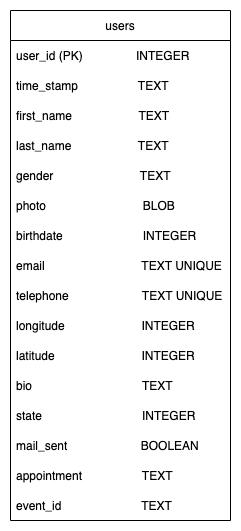
\includegraphics[width=0.5\textwidth]{images/220325_PA28464_DataBaseModel.png}
            \caption{coachingBot\_DB - Datenbankmodell}
            \label{fig: data base model}
        \end{figure}


    \section{Anbindung Datenbank an Python}
        Um eine individuelle Implementierung eines Database-Connectors zu vermeiden, bedient die Applikation sich der sqlite3-Bibliothek. Sie ermöglicht es, klassische Datenbank-Operationen direkt aus einem Python-Skript heraus anzustoßen und dient hier als Database-Connector. Die Operationen selbst werden in handelsüblichem SQL formuliert und übergeben.


    \section{Kalender}
        Um am Ende des Konversationsflusses einen ersten Termin mit einem Coach vereinbaren zu können, muss der Nutzer einen freien Termin auswählen können und für diesen eine Einladung beantragen. Zu diesem Zweck wurde die Google Calendar API angebunden. Der Nutzer wird zunächst gefragt, ob er überhaupt einen Termin vereinbaren möchte. Daraufhin wird die API abgefragt und dem Nutzer werden drei Termine vorgeschlagen. Mit einem Klick kann der gewünschte Termin dann ausgewählt werden. Kurz darauf erhält der Nutzer eine Termineinladung an die zuvor angegebene E-Mail-Adresse und kann diese im persönlichen Kalender-Client annehmen oder ablehnen. \\
        Eine Kennenlern-Sitzung dauert 50 Minuten. Vorschläge sollen über eine Spanne von 10 Tagen verteilt sein und nur an Wochentagen und zu Geschäftszeiten möglich sein. Da sich Geschäftszeiten ändern können und dazu keine Anpassung am Programmcode notwendig sein soll, werden Geschäftszeiten direkt im entsprechenden Kalender festgelegt.

    
    \section{Web-GUI}
        Um gesammelte Daten und vereinbarte Termine am Ende anzeigen zu können, wird eine einfach Web-GUI mittels HTML und CSS erstellt und auf einem lokalen Flask Web-Server deployed. Die Anbindung an die Datenbank ist bereits über den Database Connector implementiert, der auch für die Web-GUI die Daten liefert. Für eine einfache, direkte Einsicht in vereinbarte Termine, wird eine Google-Calendar View eingebunden. 